\documentclass[12pt]{report}
\usepackage[utf8]{inputenc}
\usepackage[spanish]{babel}
\usepackage{textcomp}
\usepackage{graphicx}
\usepackage{amsmath}
\usepackage{geometry}
\usepackage{colortbl}
\usepackage{array}
\usepackage{enumitem}
\geometry{left=2.5cm, right=2.5cm, top=2.5cm, bottom=2.5cm}
\usepackage{titlesec}
\usepackage[backend=biber,style=numeric,sorting=none,maxnames=5,minnames=1,doi=false,isbn=false,url=false]{biblatex}
\addbibresource{referencias.bib}
% Estilo para títulos de sección
\titleformat{\section}{\normalfont\Large\bfseries}{\thesection}{1em}{}
\usepackage{atbegshi}
\spanishdecimal{.}
\begin{document}

% Portada estilizada

    \begin{center}
    
        % Logos e institución
        
\includegraphics[width=4cm]{Reporte Semestre 1/logos/uaem.png} \hfill
        
\includegraphics[width=5cm]{Reporte Semestre 1/logos/ciicap.png} \\[2cm]
        
        % Línea separadora superior
        \hrulefill \\[0.4cm]

        % Programa educativo
        {\Large \textsc{Maestría en Ingeniería y Ciencias Aplicadas}} \\[0.5cm]

        % Título del reporte
        \hrulefill \\[0.4cm]
        {\LARGE \textbf{Trayectorias Cuánticas Difusivas Para Simular\\
        Espectros de Fluorescencia Resonante}} \\[0.4cm]
        \hrulefill \\[0.5cm]

        % Subtítulo y periodo
        {\Large \textbf{Primer Reporte Semestral}} \\[0.2cm]
        {\large \textbf{Periodo: Agosto-Diciembre 2024}} \\[2cm]
        
        \vfill

        % Información del estudiante
        \textbf{Alumno:} \\[0.2cm]
        {\Large L. T. Kevin Martínez Franco} \\[1.5cm]

        % Información del asesor
        \textbf{Asesor:} \\[0.2cm]
        {\Large Dr. Héctor Manuel Castro Beltrán} \\[2cm]

        % Fecha
        {\large \textbf{\today}} \\[2cm]
        
        % Línea final
        \hrulefill

    \end{center}


% Resumen
\section*{Resumen}

Este reporte presenta el avance en el desarrollo de simulaciones numéricas para la observación de espectros de fluorescencia de alta resolución en sistemas atómicos de uno o dos niveles. La teoría de Trayectorias Cuánticas se utiliza como marco teórico para modelar la evolución estocástica de la función de onda de estos sistemas, particularmente en configuraciones de detección heterodina y homodina, que permiten obtener espectros mucho más angostos que las líneas espectrales naturales. \\

La metodología empleada se basa en la implementación de ecuaciones estocásticas en Python utilizando el paquete QuTiP, lo cual permite simular diferentes tipos de trayectorias cuánticas. Los resultados preliminares incluyen simulaciones de Fluorescencia Resonante Intermitente (shelving) y un sistema de dos niveles, generando distribuciones de tiempos oscuros y de espera mediante la ecuación maestra y trayectorias de brincos cuánticos utilizando el método de Monte Carlo, como preámbulo para la aplicación de trayectorias difusivas.\\

Estos resultados sugieren que el uso de trayectorias cuánticas proporciona una representación eficiente y detallada de la dinámica de emisión de luz en sistemas cuánticos, con potencial para extenderse a configuraciones más complejas en el futuro. Esta investigación aporta nuevas herramientas para el estudio de espectroscopia de alta resolución y abre la puerta a una mejor comprensión de las interacciones átomo-láser en sistemas controlados experimentalmente.




% Introducción
\section*{Introducción}

La Física Atómica y la Óptica Cuántica han evolucionado hacia la manipulación precisa de sistemas a nivel de átomos e iones individuales, impulsada en gran parte por la capacidad de atraparlos en trampas que combinan campos eléctricos y magnéticos. Desde los años 1980, estas técnicas han permitido estudiar con detalle los procesos de emisión y absorción de luz. La espectroscopía de fluorescencia ha sido fundamental en estos estudios, en particular mediante la detección heterodina, donde la luz emitida se mezcla con un haz de referencia para obtener el espectro de fluorescencia.\\

En estudios previos, como los de Höffges et al.[1][2], se logró medir espectros de fluorescencia de alta resolución en sistemas de dos niveles. Estos avances han llevado al desarrollo de la Teoría de Trayectorias Cuánticas, que describe la evolución estocástica de sistemas cuánticos y permite simular mediciones como el fotoconteo y la detección heterodina.


\section*{Objetivos}

\textbf{Objetivo General:} \\
Simular sistemas cuánticos de dos y tres niveles utilizando la teoría de Trayectorias Cuánticas para estudiar fenómenos como el Fluorescencia Resonante Intermitente y la detección heterodina, obteniendo distribuciones de tiempos de espera y tiempos oscuros.\\

\textbf{Objetivos Específicos:}
\begin{itemize}
    \item Simular un sistema de tres niveles con intermitencia, analizando los efectos de este fenómeno en la dinámica del sistema.
    \item Simular un sistema de dos niveles, aplicando el modelo de trayectorias cuánticas para explorar su comportamiento estocástico.
    \item Obtener distribuciones de tiempos de espera y tiempos oscuros para ambos sistemas, utilizando la ecuación maestra y trayectorias de brincos cuánticos con el método de Monte Carlo.
    \item Simular la detección heterodina en un sistema de dos niveles, evaluando su capacidad para obtener espectros de alta resolución.
\end{itemize}



% Metodología
\section*{Metodología}

Abordamos el fenómeno de fluorescencia resonante intermitente, que describe la alternancia aleatoria entre per\'iodos de emisión frecuente de fotones ("brillantes") y periodos de nula emisión (``oscuros'') en un átomo excitado por un láser [3]. \\

Consideramos un átomo de tres niveles interactuando con un láser que excita la transici\'on 
$|e \rangle - |g \rangle$ con frecuencia de Rabi $\Omega$, y que decae a raz\'on $\gamma$, generando un per\'iodo brillante. 
\\
El estado $|e \rangle$ decae ocasionalmente a raz\'on $\gamma_d$ a un estado metaestable $|a \rangle$ que interrumpe la fluorescencia en $|e \rangle - |g \rangle$. Al decaer el estado $|a \rangle$ a $|g \rangle$ a raz\'on $\gamma_a$ vuelve la fluorescencia. Las razones de emisi\'on espont\'anea cumplen 
$\gamma \gg \gamma_d,\gamma_a$.
\\

Para simular este proceso, utilizamos el método de Trayectorias Cuánticas [4], que modela la dinámica de emisión fotónica del sistema. 
\begin{figure}
    \centering
    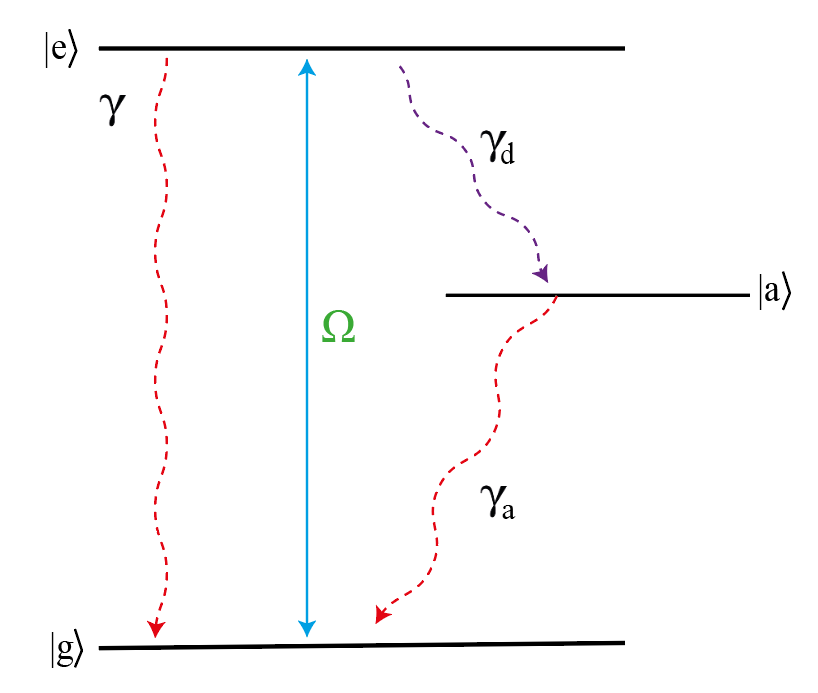
\includegraphics[width=0.5\linewidth]{1 sistema.png}
    \caption{Esquema del sistema de 3 niveles}
    \label{fig:enter-label}
\end{figure}

\\

\subsection*{Trayectorias Cuánticas}
Para simular una trayectoria cu\'antica de saltos resolvemos la ecuaci\'on de Schr\"odinger $i\hbar \dot{|\Psi \rangle} =H_{\mathrm{eff}} |\Psi \rangle$, donde $H_{\mathrm{eff}} = H - i \frac{\gamma}{2} A_{ee} -i \frac{\gamma_d}{2} A_{ee} - i \frac{\gamma_a}{2} A_{aa}$ es un Hamiltoniano efectivo no-Hermitiano, $H = \Delta A_{eg} A_{ge} + \frac{\Omega}{2} (A_{eg} + A_{ge})$ es el Hamiltoniano de la interacci\'on \'atomo-l\'aser, y los siguientes t\'erminos denotan emisi\'on espont\'anea. 

\\

Una trayectoria consiste en intervalos de evoluci\'on no unitaria hasta que se emite un fot\'on en alguna de las transiciones con 
probabilidad $p_k(t) = \delta t \langle \Psi_c(t) | \mathcal{C}_k^\dagger \mathcal{C}_k | \Psi_c(t) \rangle$, 
donde $\mathcal{C}_k = \sqrt{\gamma_k} A_{kk}$ son los operadores de colapso que representan los diferentes canales de emisión. De no emitirse un fot\'on el sistema contin\'ua siguiendo la ecuaci\'on de Schr\"odinger.
\\

El promedio en el ensamble de muchas trayectorias reproduce la evolución del operador de densidad $\rho$, que obedece la ecuación maestra $\dot{\rho} = -\frac{i}{\hbar} [H, \rho] + \mathcal{L}_D \rho$, donde $\mathcal{L}_D$ es el superoperador de Lindblad, que modela las emisiones espontáneas entre los diferentes niveles atómicos. 


\subsection*{Simulaciones}
Para llevar a cabo la simulación de sistemas cuánticos de dos y tres niveles, implementamos la teoría de Trayectorias Cuánticas, utilizando el método de Monte Carlo. Las simulaciones se desarrollaron en Python, empleando el paquete QuTiP, que permite modelar la evolución estocástica de sistemas cuánticos abiertos mediante operadores de colapso y Hamiltonianos definidos.

En el caso del sistema de tres niveles, definimos los estados base, excitado e intermedio (metastable). El estado inicial del sistema es el estado base, desde el cual pueden ocurrir transiciones hacia los otros niveles bajo la influencia de un láser con frecuencia de Rabi $\Omega$ y desintonía $\Delta$. Las transiciones posibles son de tipo brillante y oscuro, representando los periodos brillantes y oscuros característicos del fenómeno de \textit{shelving}.

Para capturar la dinámica de emisión, los operadores de colapso se definen en función de las tasas de decaimiento ($\gamma$, $\gamma_d$, $\gamma_a$) entre los estados del sistema. Estos operadores permiten modelar la interacción entre el sistema y su entorno, generando transiciones estocásticas que se resuelven con el método de Monte Carlo. El Hamiltoniano (\texttt{H}) describe la interacción láser-átomo y, junto con los operadores de colapso, define la evolución temporal del sistema. La función \texttt{mcsolve} de QuTiP se utiliza para obtener las trayectorias cuánticas correspondientes, permitiendo observar las distribuciones de tiempos brillantes y oscuros en el sistema.\\

Para el sistema de dos niveles, el procedimiento es similar pero con menos transiciones posibles, ya que solo considera los estados base y excitado. Esto simplifica la configuración de los operadores y permite un análisis directo de las transiciones brillantes y oscuros en el sistema, obteniendo distribuciones de tiempos de espera y tiempos oscuros que ayudan a caracterizar la dinámica del sistema.
\\
\\
\subsection*{Distribución de tiempos oscuros}\\

El procedimiento de c\'alculo de trayectorias permite recoger la informaci\'on de fotoemisiones y estad\'istica de los per\'iodos brillantes y oscuros[3]. Esto se logra mejor si hacemos una trayectoria muy larga en lugar de muchas trayectorias cortas. Se pueden obtener las distribuciones de las duraciones de los periodos oscuros y brillantes, que siguen distribuciones exponenciales: 
$$ P_O = \frac{1}{T_O} e^{-t/T_O}, \qquad  
    P_B = \frac{1}{T_B} e^{-t/T_B} ,$$
con duraciones promedio
$$ T_O = \gamma_a^{-1}, \qquad T_B = \frac{2\Omega^2 + \gamma^2 + 4\Delta^2}{\gamma_d \Omega^2} .$$
\\
\textbf{Algoritmo para realizar la distribución de tiempos oscuros con los resultados obtenidos de la simulación}
\begin{enumerate} \item \textbf{Registro de Eventos de Colapso} \begin{itemize} \item Durante la simulación, se registran eventos de colapso en ciertos tiempos. \item Cada colapso corresponde a una transición específica en el sistema. \end{itemize} \vspace{0.5em} \item \textbf{Identificación de Períodos} \begin{itemize} \item \textbf{Períodos Brillantes}: Intervalos donde el sistema emite fluorescencia. \item \textbf{Períodos Oscuros}: Intervalos donde no hay emisión de fluorescencia. \end{itemize} \vspace{0.5em} \item \textbf{Detección de Transiciones Clave} \begin{itemize} \item Se enfocan en colapsos específicos que marcan el inicio y fin de los períodos. \item Por ejemplo, un colapso de tipo 1 indica el inicio de un período brillante. \end{itemize} \vspace{0.5em} \item \textbf{Cálculo de Duraciones} \begin{itemize} \item \textbf{Períodos Brillantes}: Duración = tiempo de fin - tiempo de inicio. \item \textbf{Períodos Oscuros}: Duración = inicio del siguiente período brillante - fin del período brillante actual. \end{itemize} \vspace{0.5em} \item \textbf{Almacenamiento y Análisis} \begin{itemize} \item Se guardan las duraciones para análisis estadístico. \item Permite calcular tiempos promedio y visualizar patrones de intermitencia. \end{itemize} \end{enumerate}

\subsubsection*{Distribución de Tiempos de Espera en el Sistema de Tres Niveles}

En la simulación del sistema de tres niveles, se modela la probabilidad de contar eventos de fotoconteo en función del tiempo. Esta probabilidad se describe mediante una distribución de Poisson, que permite calcular la probabilidad de que se emitan \( n \) fotones en un intervalo de tiempo \( T \). Bajo una intensidad de campo constante, la probabilidad de detectar \( n \) fotoelectrones es:
%
\begin{equation}
p(n, T) = \frac{(\xi \bar{I} T)^n}{n!} e^{-\xi \bar{I} T},
\end{equation}
%
donde $\xi$ es la eficiencia de detección $\bar{I}$ es la intensidad media del campo incidente. Este enfoque permite analizar la distribución de tiempos de espera entre eventos de emisión, considerando tanto el régimen de dos niveles (\( |g\rangle \) y \( |e\rangle \)) como los períodos oscuros asociados al estado metastable \( |m\rangle \).



La tasa de decaimiento del estado excitado al estado metastable, \( \gamma_{m} \), afecta directamente la frecuencia con la que el sistema entra en períodos oscuros. Una tasa de decaimiento más alta incrementa el número de períodos oscuros en la distribución final de tiempos de espera, y contribuye a la complejidad de la dinámica de fluorescencia intermitente. La distribución de tiempos de espera con períodos oscuros puede analizarse usando:
\begin{equation
w(\tau) = \frac{1}{\tau_0} e^{-\tau/\tau_0},
\end{equation}
donde \( \tau_0 \) es el tiempo medio entre eventos de fotoconteo. Este resultado, conocido como la función de retardo, es útil para modelar la fluorescencia resonante y analizar la duración de los períodos oscuros en el sistema, ya que describe la probabilidad de no detectar un fotón durante el retardo \( \tau \).
 

% Resultados
\section*{Resultados Preliminares}
\subsection*{Simulación del Sistema de Tres Niveles}

En esta sección presentamos los resultados de las simulaciones realizadas en el sistema de tres niveles, en el que estudiamos las distribuciones de tiempos brillantes y oscuros mediante trayectorias cuánticas. Estas simulaciones permiten observar el fenómeno de \textit{shelving}, donde el sistema pasa por períodos brillantes con oscilaciones de Rabi y períodos oscuros debido a la transición hacia un estado metastable.

En la Fig. 2, a la izquierda, mostramos un fragmento de una trayectoria típica del sistema, destacando los períodos brillantes con oscilaciones de Rabi y los períodos oscuros característicos. A la derecha, presentamos el promedio de un ensamble de 4000 trayectorias, que se compara favorablemente con el resultado obtenido mediante la ecuación maestra. Los parámetros utilizados fueron $\Omega=3.5\gamma$, $\Delta=0$, $\gamma_d=0.95\gamma$, $\gamma_d=0.05\gamma$, y $\gamma_a =0.015 \gamma$.

\begin{figure}[t]
    \centering
    
\includegraphics[width=0.9\linewidth]{Reporte Semestre 1/zoom y meq vs tj.png}
    \caption{A la izquierda: Fragmento de la población del estado excitado de una trayectoria. A la derecha: Promedio en un ensamble de 4000 trayectorias, comparado con el resultado obtenido mediante la ecuación maestra.}
\end{figure}
\begin{figure}[!]
    \centering
    
\includegraphics[width=0.5\linewidth]{Reporte Semestre 1/descarga (1).png}
    \caption{Gráfica de los períodos oscuros a lo largo de la simulación: el eje $x$ representa el tiempo de ocurrencia de cada período oscuro, y el eje $y$ su duración. Esta visualización permite observar la variabilidad en la duración y distribución temporal de los períodos oscuros en la simulación de $10^6 \gamma^{-1}$.}
\end{figure}

\begin{figure}[h]
    \centering
    
\includegraphics[width=0.6\linewidth]{Reporte Semestre 1/descarga.png}
    \caption{Histograma de los períodos oscuros obtenidos de las simulaciones (en magenta) y distribución teórica escalada $P_O(t)$ (curva negra) con parámetros ajustados en función de los bins y el número total de períodos oscuros observados.}
\end{figure}


En un per\'iodo brillante la raz\'on de emisi\'on de fotones es $\gamma \langle \rho_{ee} (t) \rangle$. Un per\'iodo oscuro finaliza cuando se vuelve a emitir un fot\'on en la transici\'on fuerte, iniciando otro per\'iodo brillante. Estos per\'iodos ocurren estoc\'asticamente. 
\subsection*{Distribución Temporal de los Períodos Oscuros}

La Fig. 3 presenta una gráfica que muestra el tiempo de ocurrencia (eje $x$) y la duración (eje $y$) de cada período oscuro a lo largo de la simulación, la cual abarca un tiempo total de $10^6 \gamma^{-1}$. Esta representación permite observar la dispersión en la duración de los períodos oscuros y su distribución temporal durante la evolución del sistema.

Cada barra en la gráfica corresponde a un período oscuro específico, con su posición en el tiempo en el eje $x$ y su duración en el eje $y$. Esto proporciona una visualización clara de cómo los períodos oscuros se distribuyen a lo largo de la simulación, resaltando tanto la variabilidad en su duración como la frecuencia de su aparición. Este análisis temporal es útil para identificar patrones o tendencias en la dinámica de \textit{shelving} del sistema de tres niveles, donde los períodos oscuros se alternan con períodos brillantes.



\subsection*{Distribución de Tiempos Oscuros}

En la Fig. 4, mostramos el histograma de los períodos oscuros obtenido de las simulaciones del sistema de tres niveles. La duración promedio teórica de estos períodos oscuros, $T_{oc}$, se calcula como el inverso de la tasa de decaimiento hacia el estado metastable, es decir, $T_{oc} = 1/\gamma_a$. Para comparar los resultados simulados con la teoría, ajustamos la distribución teórica en función de los bins y el número total de períodos oscuros observados en las simulaciones. 

La distribución teórica escalada $P_O(t)$, representada por la curva negra en la gráfica, muestra un buen ajuste con el histograma de los datos simulados. Este ajuste permite verificar la consistencia entre los resultados de las simulaciones y la teoría en cuanto a la duración y frecuencia de los períodos oscuros, proporcionando un análisis cuantitativo de estos eventos en el sistema de tres niveles.




\subsection*{Distribuciones de Tiempos de Espera del Sistema de Tres Niveles}

La dinámica del sistema de tres niveles implica dos tipos de transiciones principales: las transiciones entre los estados \( |g\rangle \) y \( |e\rangle \), que se comportan como un sistema de dos niveles, y las transiciones hacia y desde el estado metastable \( |m\rangle \), que introducen períodos oscuros (momentos sin emisión de fotones). Estos períodos oscuros ocurren cuando el sistema entra en el estado metastable y se mantiene en él antes de regresar al ciclo de emisión de fotones.

En las figuras a continuación, mostramos las distribuciones de tiempos de espera para dos configuraciones de la frecuencia de Rabi. En ambas figuras, la gráfica de la izquierda muestra la distribución de tiempos de espera para las transiciones \( |e\rangle \rightarrow |g\rangle \), representando el comportamiento de un sistema de dos niveles sin la influencia del estado metastable. La gráfica de la derecha muestra la distribución total de tiempos de espera, que incluye el efecto del \textit{shelving} (estado metastable). Esta gráfica está recortada en el eje $x$ con un límite de 20 para visualizar mejor la estructura principal de la distribución, aunque existen tiempos de espera que alcanzan hasta 450 unidades de duración.

La frecuencia de Rabi, denotada por \( \Omega \), tiene un impacto significativo en la dinámica del sistema. En la Fig. \ref{fig:dist_rabi_1}, la frecuencia de Rabi es baja (\( \Omega = 1 \gamma \)), lo que produce una menor interacción entre los estados, afectando la frecuencia y duración de los períodos oscuros en la distribución total. En la Fig. \ref{fig:dist_rabi_3.5}, con una frecuencia de Rabi más alta (\( \Omega = 3.5 \gamma \)), se observa un incremento en la tasa de transiciones, lo cual modifica la estructura de las distribuciones.

\begin{figure}[h]
    \centering
    
\includegraphics[width=1\linewidth]{Reporte Semestre 1/Debil.png}

    \caption{Distribuciones de tiempos de espera para el sistema de tres niveles con frecuencia de Rabi \( \Omega = 1 \gamma \): (izquierda) distribución de tiempos de espera para las transiciones \( |e\rangle \rightarrow |g\rangle \) sin el estado metastable; (derecha) distribución total de tiempos de espera, incluyendo el efecto del \textit{shelving}, recortada a un límite de 20 en el eje $x$ para mejorar la visualización.}
    \label{fig:dist_rabi_1}
\end{figure}

\begin{figure}[h]
    \centering
    
\includegraphics[width=1.01\linewidth]{Reporte Semestre 1/Fuerte.png}

    \caption{Distribuciones de tiempos de espera para el sistema de tres niveles con frecuencia de Rabi \( \Omega = 3.5 \gamma \): (izquierda) distribución de tiempos de espera para las transiciones \( |e\rangle \rightarrow |g\rangle \) sin el estado metastable; (derecha) distribución total de tiempos de espera, incluyendo el efecto del \textit{shelving}, recortada a un límite de 20 en el eje $x$ para mejorar la visualización.}
    \label{fig:dist_rabi_3.5}
\end{figure}

%Trabajo Futuro
\section*{Perspectiva del segundo semestre}
El objetivo en el siguiente semestre es simular el espectro del sistema, Fig. 7, con detección heterodina usando trayectorias cuánticas difusivas. Usar brincos nos ayudo a hacer un análisis preliminar a partir con foto conteo, cosa que no se puede hacer con detección heterodina por la intensidad alta del oscilador local.[1][2]\\

La detección heterodina tiene la capacidad de resolver espectros del orden de Hz, mientras que un filtro Fabryt-Perot 
en contraste tiene resoluciones del orden de KHz.[5].




\begin{figure}[h]
    \centering
    
\includegraphics[width=0.7\linewidth]{Reporte Semestre 1/hoffges E angosto.png}
    \caption{Espectro esperado que presenta un pico angosto, simulable mediante trayectorias cuánticas difusivas. Este resultado permitirá estudiar espectros de alta resolución en sistemas abiertos.}
    \label{fig:espectro_futuro}
\end{figure}

\begin{figure}[!]
    \centering
    
\includegraphics[width=0.7\linewidth]{Reporte Semestre 1/deteccion h.png}
    \caption{Esquema de la detección heterodina}
    \label{fig:enter-label}
\end{figure}

% Anexos
\section*{Anexos}

\subsection*{Participación en el Workshop on Open Quantum Systems and Quantum Information}

Asistí al \textit{Workshop on Open Quantum Systems and Quantum Information} en Puebla, organizado por el Instituto de Física de la BUAP del 15 al 19 de julio de 2024. Este evento reunió a investigadores y estudiantes de diversas áreas de la física cuántica, abordando temas como sistemas cuánticos abiertos, información cuántica, entrelazamiento cuántico, interacción luz-materia, y teoría de matrices aleatorias aplicada a sistemas de muchos cuerpos. Más información sobre el evento se encuentra en su página oficial: \url{https://www.ifuap.buap.mx/eventos/2024/quantum/}.

En el workshop, presenté un póster titulado "Trayectorias Cuánticas Difusivas para Simular Espectros de Fluorescencia Resonante," el cual resume los objetivos y avances de mi proyecto de investigación. A continuación, se incluye la constancia de participación otorgada por los organizadores y una copia del póster presentado.

\begin{figure}[h]
    \centering
    
\includegraphics[width=0.8\linewidth]{Reporte Semestre 1/constancia.png}
    \caption{Constancia de participación en el \textit{Workshop on Open Quantum Systems and Quantum Information}.}
\end{figure}

\begin{figure}[I]
    \centering
    \includegraphics[width=0.8\linewidth]{Reporte Semestre 1/posterpdf_page-0001.jpg}
    \caption{Póster presentado en el \textit{Workshop on Open Quantum Systems and Quantum Information}, titulado "Trayectorias Cuánticas Difusivas para Simular Espectros de Fluorescencia Resonante".}
\end{figure}

\newpage
\subsection*{Cronograma de actividades}
\begin{document}

\begin{table}[h!]
\centering
\renewcommand{\arraystretch}{1.5}
\begin{tabular}{|p{9cm}|c|c|c|c|}
\hline
\textbf{Actividad} & \multicolumn{4}{c|}{\textbf{Semestre}} \\ \cline{2-5} 
 & 1 & 2 & 3 & 4 \\ \hline
Búsqueda de información y análisis del estado del Arte & \cellcolor{green} & & & \\ \hline
Estudio detallado de ecuaciones maestras y teoría de trayectorias cuánticas & \cellcolor{green} & & & \\ \hline
Definición del marco teórico y planteamiento del problema & \cellcolor{green} & & & \\ \hline
Definición de la metodología de simulación numérica (trayectorias cuánticas) & & \cellcolor{green} & & \\ \hline
Selección y adaptación de herramientas computacionales (QuTiP, Python) & & \cellcolor{green} & & \\ \hline
Elaboración del diseño de simulación (condiciones iniciales, parámetros, algoritmos) & & \cellcolor{green} & & \\ \hline
Programación de simulaciones de trayectorias cuánticas para sistemas simples & & \cellcolor{green} & & \\ \hline
Simulación y ajuste de parámetros (ejecución y depuración de código) & & \cellcolor{green} & & \\ \hline
Análisis preliminar de resultados de simulaciones & & \cellcolor{green} & & \\ \hline
Comparación con experimentos previos y ecuaciones maestras & & & \cellcolor{green} & \\ \hline
Validación y ajuste de modelos teóricos & & & \cellcolor{green} & \\ \hline
Discusión de resultados, refinamiento de hipótesis & & & \cellcolor{green} & \\ \hline
Redacción del informe de investigación (marco teórico, metodología, resultados) & & & \cellcolor{green} & \cellcolor{green} \\ \hline
Preparación de presentaciones para congresos o seminarios & & & & \cellcolor{green} \\ \hline
Defensa del proyecto & & & & \cellcolor{green} \\ \hline
\end{tabular}
\end{table}

\newpage
\section*{Bibliografia}
\begin{enumerate}
    \item J. T. Höffges, H. W. Baldauf, T. Eichler, S. R. Helmfrid, and H. Walther, Opt. Commun. \textbf{133}, 170 (1997).
    \item J. T. Höffges, H. W. Baldauf, W. Lange, and H. Walther, J. Mod. Opt. \textbf{44}, 1099 (1997).
    \item H. J. Carmichael, \textit{An Open Systems Approach to Quantum Optics} (Springer, Berlin, 1993).
    \item M. B. Plenio and P. L. Knight, Rev. Mod. Phys. \textbf{70}, 101 (1998).
    \item V. Bühner and Ch. Tamm, Phys. Rev. A \textbf{61}, 061801 (2000).
    \item H. J. Carmichael, in \textit{Coherence and Quantum Optics VII}, edited by J. H. Eberly, L. Mandel, and E. Wolf (Plenum Press, New York, 1996), p. 177.
\end{enumerate}

\end{document}
\end{document}


